%%
%% 2015-11-03 -UK- aktualisiert
%% ====================================================================
\documentclass[pamm,a4paper,fleqn]{w-art}
\usepackage{times,cite,w-thm}
\usepackage[T1]{fontenc}
\usepackage[utf8]{inputenc}
%% By default the equations are consecutively numbered. This may be changed by
%% the following command.
%% \numberwithin{equation}{section}
%%
%%
%% The usage of multiple languages is possible.
%% \usepackage{ngerman}% or
%% \usepackage[english,ngerman]{babel}
%% \usepackage[english,french]{babel}
\usepackage{graphicx}

\usepackage{amsmath}
\usepackage{amssymb}

%-------------------------------------------------------------------------------
% Useful mathematical macros
\newcommand{\Data}{\vec{D}}
\newcommand{\DataExt}{\widetilde{\vec{D}}}
\newcommand{\MSE}{\ensuremath{\text{MSE}}}
\newcommand{\T}{\ensuremath{\text{T}}}
\renewcommand{\vec}[1]{\boldsymbol{#1}}
\newcommand{\mat}[1]{\boldsymbol{#1}}
\newcommand{\VTheta}{\ensuremath{\vec{\theta}}}
\newcommand{\VLambda}{\ensuremath{\vec{\lambda}}}
\DeclareMathOperator*{\argmin}{arg\,min}
\newcommand{\R}{\mathbb R}
\newcommand{\UNN}[1][\text{NN}]{u_{#1}}
\newcommand{\FNN}[1][\text{NN}]{f_{#1}}
\newcommand{\NonlinOp}{\mathcal N\!}
\newcommand{\norm}[1]{\left\lVert#1\right\rVert}
% -------------------------------------------------------------------------------

%% 
\begin{document}
%% \def\leftmark{Session title}
%%
%%    The information for the title page will be placed between
%%    \begin{document} and \maketitle. The order of most entries
%%    is determined by the class file and cannot be changed by
%%    rearranging them. The maketitle command follows after the
%%    abstract.
%%
%%    The following commands will be updated by the publisher:
%%
%%    \renewcommand{\copyrightyear}{2016}
%%    \DOIsuffix{pamm.20161zzzz}
%%    \Volume{16} 
%%    \Year{2016} 
%%    \pagespan{1}{}
%%
%%    The short title is optional:

\TitleLanguage[EN]
\title[Divergence-free neural networks]{Estimating divergence-free flows via
  neural networks}

%% Please delete not needed author entries.
%% Information for the first author.
\author{\firstname{Dmitry I.} \lastname{Kabanov}\inst{1,}%
\footnote{Corresponding author:
  e-mail \ElectronicMail{kabanov@uq.rwth-aachen.de}.}} 
%%
%%    Information for the second author
\author{\firstname{Luis} \lastname{Espath}\inst{1}}
%%
%%    Information for the third author
\author{\firstname{Jonas} \lastname{Kiessling}\inst{2}}
\author{\firstname{Raul F.} \lastname{Tempone}\inst{1,3}}

\address[\inst{1}]{\CountryCode[DE]RWTH Aachen University, Pontdriesch 14--16,
  Aachen 52062, Germany}
\address[\inst{2}]{\CountryCode[SE]KTH Royal Institute of Technology,
  SE-100 44 Stockholm, Sweden}
\address[\inst{3}]{\CountryCode[SA]King Abdullah University of Science and
  Technology, Thuwal, 23955-6900, Saudi Arabia}
%%
%%    \dedicatory{This is a dedicatory.}
%%
%%    Abstract is required.
\AbstractLanguage[EN]
\begin{abstract}
We apply neural networks to the problem of estimating divergence-free flows from
given sparse observations.
Following modern trend of combining data and models together to obtain
physics-informed neural networks, we reconstruct the flow by training a neural
network in such manner that it not
only matches the observations but also approximately satisfies the
incompressibility condition.
The balance between two terms is found through a cross-validation procedure.
We apply this
approach to synthetic dataset with truly divergence-free flow and to wind
reconstruction over Sweden.
\end{abstract}
%% maketitle must follow the abstract.
\maketitle                   % Produces the title.

\section{Introduction}

An important method of finding relations from given dataset of observations
is through fitting a function to this dataset.
The function should be ``rich'' enough so that the relations between independent
and dependent variables in the dataset can be modeled properly.
Recently, special nonlinear functions called neural networks have emerged for
the purpose of finding relations in the data, particularly, an important class
of functions named \emph{physics-informed neural networks} \cite{RaissiEtAl2019} has emerged for
the purposes of fitting the data, for which one can postulate important physical
properties of this data.

We apply physics-informed neural networks to the problem of estimating flows
with divergence-free property, namely, flows of incompressible fluids.
For that, we train the network to not only satisfy the given dataset of
observations but also to approximately satisfy the divergence-free condition.

We demonstrate the performance of such networks on two examples.
One example is based on the truly divergence-free data.
The second example is based on the dataset of wind velocity observations over
Sweden in 2018, where we use an assumption that the wind is incompressible due
to the relatively low wind velocities.

\section{Mathematical model}
Consider dataset
\begin{equation}
  \label{eq:dset}
  \vec{D} = \left\{\vec{x}_i, \vec{u}_i\right\}, \quad i = 1, \dots, N
\end{equation}
where $\vec{x}_i = (x_i, y_i) \in \mathcal D \subset \R^2$ is a spatial point,
$\vec{u}_i = (u_i, v_i) \in \R^2$ is the velocity field at point $i$.
Also, assume that the velocity field $\vec u (\vec x)$ satisfies the
divergence-free condition, at least approximately:
\begin{equation}
  \label{eq:div-free}
  \nabla \cdot \vec u (\vec x) \approx 0.
\end{equation}
We seek an estimator $\hat{\vec u} (\vec x; \vec \theta)\approx \vec u(\vec x)$
parameterized by $\vec \theta \in \R^n$ that satisfies
the measurements~\eqref{eq:dset} and the divergence-free
condition~\eqref{eq:div-free} simultaneously
\begin{equation}
  \label{eq:opt-problem}
  \arg \min_\theta \quad
  \frac{1}{N} \sum_{i=1}^N \norm{\vec u_i - \hat{\vec u}(\vec x_i; \vec\theta)}^2_2
  \ + \ 
  \frac{\gamma}{P} \sum_{i=1}^P \left( \nabla \cdot \hat{\vec u}(\vec x_i; \vec\theta)\right)^2
\end{equation}
where 
$\gamma$ is regularization parameter that determines how strongly
the divergence-free condition is enforced, 
and $P$ points, at which the divergence-free condition is enforced, are different
from the measurement locations.

As an estimator function $\hat{\vec u}(\vec x; \theta)$, we use a neural network
of type ``multilayer perceptron''\cite{GoodfellowEtAl2016}, which is trained
(that is, parameter $\vec\theta$ is fitted) by solving 
the optimization problem~\eqref{eq:opt-problem} via ADAM
optimizer~\cite{KingmaBa2014}.
Also, iterations of $\vec\theta$ are averaged using exponential
averaging, and the averaged value is used for making predictions with the
trained model.

\section{Numerical examples}

\textbf{Example 1}.
We generate synthetic noiseless data
  $\left\{(x_i, y_i), \vec{u}_i\right\}$, $i = 1, \dots, 10$,
where $\vec u(x, y) = ( \cos x \, \sin y, -\sin x \, \cos y)^\T$
and points $(x_i, y_i)$ are sampled uniformly from domain $[0; 2\pi]^2$.
This dataset is a Taylor--Green 2D vortex fixed in time.
Test data are located on the $21\times21$ uniform grid in this domain.

Figure~\ref{fig:tg2d} shows the comparison of the prediction errors of two
networks: for one, parameter $\gamma$ is set to zero, such that the network is
trained to only match the dataset, for another, parameter $\gamma = 10^{-2}$.
We can see that the neural network trained to satisfy both  the dataset and the
divergence-free condition, gives smaller prediction errors, especially at
locations at distance from the measurement locations.

\begin{figure}
\begin{minipage}{0.48\textwidth}
  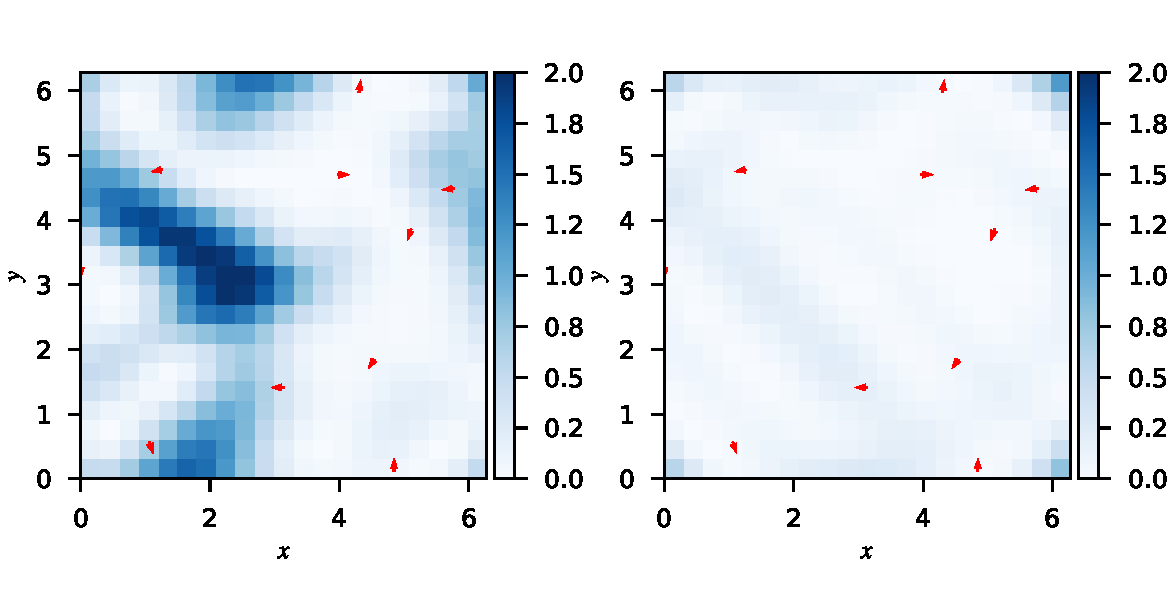
\includegraphics[width=3.3in]{assets/error-fields-comparison.pdf}
  \caption{Comparison of the prediction errors for two neural networks:
    a) $\gamma=0$; b) $\gamma=10^{-2}$.
    Red arrows show the measurement locations and corresponding
  velocity directions.}%
  \label{fig:tg2d}
\end{minipage}
\hfill
\begin{minipage}{0.48\textwidth}
  \centering
  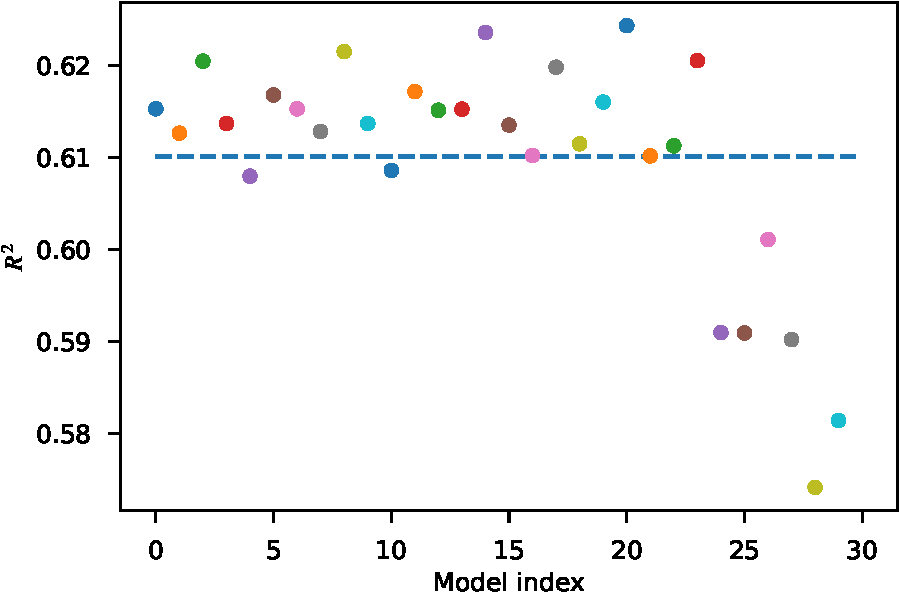
\includegraphics[scale=0.42]{assets/r2-vs-model.pdf}
  \caption{Comparison of 30 neural-network models (points)
    with the base IDW model (dashed line).
  The best found model corresponds to model index 21.}%
  \label{fig:r2-vs-model}
\end{minipage}
\end{figure}

\textbf{Example 2}.
We apply a neural network with div-free regularization to the problem of
reconstruction of the wind fields over Sweden.
The data are collected from 165 weather stations in 2018, with measurements
collected hourly but a lot of missing data points from different stations.

As the base model, we use Inverse Distance Weighting (IDW)
model~\cite{Cellura2008}, which
estimates velocity at point $\vec x_j$ by averaging weighted observations:
\begin{equation}
  \label{eq:base-model}
  \hat{\vec u}_{\text{IDW}}(\vec x_j) =
  \frac{\sum_{i=1}^N W(r_{i,j}) \vec u(\vec x_j)}{\sum_{i=1}^N W(r_{i,j})}
\end{equation}
where $W$ is a weight, namely, decaying function of the distance $r_{i, j}$.

To assess the quality of the model, we estimate the prediction error
by selecting at random from the dataset T time snapshots and computing
an average $R^2$ score using five-fold cross-validation:
\[
  R^2 = 1 - \frac{%
    \sum_{i=1}^T \sum_{j=1}^K \frac{1}{N_{ij}'}
    \sum_{k=1}^{N_{ij}'} \norm{\vec{u}_{ijk} - \hat{\vec{u}}_{ijk}}^2_2}
  {%
    \sum_{i=1}^T \sum_{j=1}^K \frac{1}{N_{ij}'}
    \sum_{k=1}^{N_{ij}'} \norm{\vec{u}_{ijk}}^2_2}
\]
where $N_{ij}'$ denotes number of test measurements for the $i$th time snapshot
and $j$th cross-validation fold.
We choose $T=500$ and $K=5$, therefore, to compute $R^2$ score 2500 neural
networks are required with a given configuration of hyperparameters.

We train neural networks with the configuration specified by a triplet: 
$\gamma \in \{0, 10^{-4}, 10^{-3}, 10^{-2}, 10^{-1}\}$, 
number of neurons in the 1st hidden layer: $h_1 \in \{20, 30\}$,
number of neurons in the 2nd hidden layer: $h_2 \in \{0, 10, 20\}$.

Figure~\ref{fig:r2-vs-model} shows comparison of the neural networks with these
configurations against the base model~\eqref{eq:base-model}.
The best $R^2$ score is achieved by the model 21 with parameters $\gamma=0.01$,
$h_1=20$, $h_2=20$.
However, one can see that the $R^2=62.5$ of the best model is relatively close
to the $R^2=0.61$ of the base model.

\section{Conclusions}

We applied physics-informed neural networks to estimation of divergence-free
flows.
Application to the synthetic data, which are known to be truly divergence-free,
shows that the addition of the divergence-free regularization significantly
improves the prediction error of the neural network, particularly, in the areas
with know measurement data.
Application to the wind estimation over Sweden shows that divergence-free neural
network can achieve better, although marginally, prediction performance than
the base inverse distaince weighting model.
Overall, addition of the physics regularizer improves the prediction performance
of neural networks.

\begin{acknowledgement}
  The authors greatfully acknowledge research funding from the Alexander von
  Humboldt Foundation.
\end{acknowledgement}

\vspace{\baselineskip}
%% The style of the following references should be used in all documents.

\begin{thebibliography}{1}

\bibitem{RaissiEtAl2019}
  M.~Raissi, P.~Perdikaris, and G.\,E.~Karniadakis.
  J. Comput. Phys. \textbf{378}, 686-707 (2019).

\bibitem{Cellura2008}
  M.~Cellura, G.~Cirrincione, A.~Marvuglia, A.~Miraoui.
  Renew. Energ., \textbf{33}, 1251-1266 (2008).

\bibitem{KingmaBa2014}
  D.\,P.~Kingma, J.~Ba.
  arXiv preprint, arXiv:1412.6980 (2014).

\bibitem{GoodfellowEtAl2016}
  I.~Goodfellow, Y.~Bengio, and A.~Courville.
  Deep Learning (MIT Press, 2016).

\end{thebibliography}

\end{document}               % End of document.
%%
%% End of file `pamm-stpl.tex'.
